\documentclass[12pt,oneside,letterpaper]{PSUreport}
\usepackage{PSUthesis}
\usepackage[pdftex]{graphicx}
\usepackage{hyperref}
\usepackage[acronym,toc]{glossaries}

\makenoidxglossaries
\newacronym{sgx}{SGX}{Software Guard Extensions}
\newacronym{tpm}{TPM}{Trusted Platform Module}
\newacronym{txt}{TXT}{Trusted Execution Technology}
\newacronym{rot}{RoT}{Root of Trust}
\newacronym{tcb}{TCB}{Trusted Compute Base}
\newacronym{prm}{PRM}{Processor Reserved Memory}
\newacronym{smm}{SMM}{System Management Mode}
\newacronym{dma}{DMA}{Direct Memory Access}
\newacronym{epc}{EPC}{Enclave Page Cache}
\newacronym{aex}{AEX}{Asynchronous Enclave Exit}
\newacronym{soc}{SoC}{System on Chip}
\newacronym{amba}{AMBA}{Advanced Microcontroller Bus Architecture}
\newacronym{axi}{AXI}{Advanced eXtensible Interface}
\newacronym{msr}{MSR}{model-specific register}
\newacronym{tfa}{TF-A}{Trusted Firmware-A}
\newacronym{optee}{OP-TEE}{Open-source Portable TEE}

\begin{document}
\title{An Overview of Trusted Execution Environments}
\subtitle{}
\author{Stephano Cetola}
\principaladviser{Prof. John Aken}             % Principal advisor
\firstreader{Prof. Marek A. Perkowski}                           % First member
\secondreader{Prof. Eric Wan}                % Second member
\deptchair{Prof. James McNames}                        % Dept. Chair
\submitdate{\today}                                    % Submission date
\submityear{2021}                                      % Just do it!

\copyrightfalse
\figurespagefalse
\tablespagefalse
\null\vfill
\begin{center}
        \copyright\ 2020 Stephano Cetola \\
        This work is licensed under the Creative Commons Attribution 4.0 International License. To view a copy of this license, visit \url{http://creativecommons.org/licenses/by/4.0/}.
\end{center}
\begin{center}
\includegraphics{./img/by.eps}
\end{center}
\vfill\newpage
 
\beforepreface
\prefacesection{Preface}
This thesis tells you all you need to know about...
\prefacesection{Acknowledgments}
I would like to thank...
\afterpreface

\printnoidxglossary[type=\acronymtype]

%==============================================================================
% Chapters
%==============================================================================
\glsresetall
\chapter{Introduction}
\pagenumbering{arabic}
\section{Problem Statement}
Historically, computer architecture security relied on processor modes or privilege modes where code was allowed to execute. In these modes, separation of privileges is achieved and often referred to as ``rings'' with ``ring 0'' being the most privileged (machine mode, kernel code) and ring 3 being the least privileged (user mode, application code). Device drivers run in the rings between these two modes with virtualization being the most common use case\footnote{The virtual machine’s kernel, for example, runs in ring 1, one level up from machine mode.}. As applications became more complex, specifically with the advent of large-scale virtualization and the internet, this simple security model broke down as executed code could no longer be trusted, nor its origin verified. The problem of ``secure remote computation'' arises where the data owner must trust not only the software provider, but also the remote computer and infrastructure on which that software is executed. Homomorphic encryption solves this problem to some extent, however the performance overhead of this transaction limits its application \cite{Gentry01}. 

In an attempt to address these issues, microprocessor designers have implemented versions of a \gls{tee}, first defined by the Open Mobile Terminal Platform and ratified in 2009 \cite{OMTP01}. The OMTP standard was transferred to the Wholesale Applications Community (WAC) in 2010 and in July 2012 WAC itself was closed, with the OMTP standards being transferred to The GSM Association (originally Groupe Spécial Mobile)\cite{WAC}. In this paper we will discuss the two most prevalent implementations of this standard for the x86-64 and AArch64 architectures, as well as a completely open source hardware and software implementation of a TEE for the RISC-V architecture.
\section{The Intel SGX Solution}
Intel \gls{sgx} is built on designs of software attestation already proven in technologies like the \gls{tpm} and Intel \gls{txt}. In \gls{sgx}, these concepts of software attestation are used to create containerized sections of memory on the remote computer called ``secure enclaves'' where data and code can be loaded or executed securely. These enclaves are verified by both a cryptographic attestation key of the container’s contents as well as a hardware \gls{rot} manufacturer’s key. Unlike the \gls{tpm} and \gls{txt} technologies, \gls{sgx} securely operates only on a small amount of data and code called the \gls{tcb}, leaving the majority of memory outside this \gls{tcb}.
\section{Initial SGX Enclave Setup}
Configuration settings for \gls{sgx} exists as part of the platform firmware, and most firmware vendors provide simple tools for enabling \gls{sgx}. If \gls{sgx} is enabled, the firmware is responsible for setting aside a memory region called the \gls{prm}, and most firmware tools allow specifying the size of the space allocated. The firmware allocates the \gls{prm} by setting a pair of \glspl{msr}, collectively known as the PRMRR. The CPU will then protect the \gls{prm} from all non-enclave memory accesses including kernel, hypervisor and \gls{smm} accesses, as well as \gls{dma} from peripherals \cite{intel-sgx-explained}. 

This section of specially allocated memory is used to store the \gls{epc}, which are the 4kb pages holding both the enclave data and code. The exact layout of the \gls{prm} and \gls{epc} are model-specific, and depend on firmware settings. While untrusted system software both assigns these EPCs to an enclave and loads them with data, it is the CPU which keeps track of all the \gls{epc}s ensuring that they only belong to one enclave. Once the system software loads data into the enclave it asks the CPU to mark that enclave as initialized, after which no other data may be loaded into the enclave as this setup process is disabled for that enclave. After initialization, this enclave is measured by a cryptographic hash to ensure that any operations performed on the enclave are done so in a secure environment.
\vspace{10 mm}

\begin{figure}[htbp]
\centering
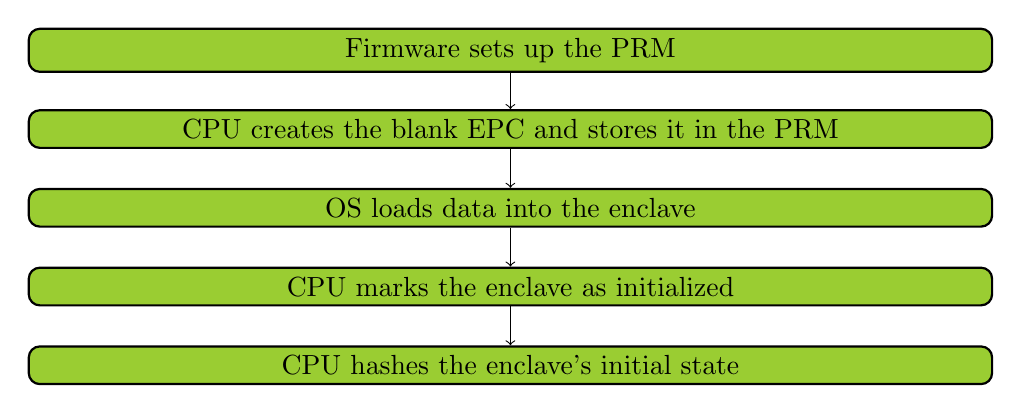
\begin{tikzpicture}[
    block/.style ={rectangle, draw=black, thick, fill=YellowGreen,
          text width=12cm, text centered, rounded corners},
    line/.style ={draw, ->}
]

\node[block] (s1) at (0,0) {Firmware sets up the PRM};
\node[block, below of = s1] (s3) {CPU creates the blank EPC and stores it in the PRM};
\node[block, below of = s3] (s5) {OS loads data into the enclave};
\node[block, below of = s5] (s10) {CPU marks the enclave as initialized};
\node[block, below of = s10] (s15) {CPU hashes the enclave’s initial state};

\path [line] (s1) -- (s3);
\path [line] (s3) -- (s5);
\path [line] (s5) -- (s10);
\path [line] (s10) -- (s15);

\end{tikzpicture}

\caption[Setting Up Intel SGX]{\textbf{Workflow for setting up an enclave.}}
\label{fig:sgx-setup}
\end{figure}

\section{Executing SGX Enclave Code}
Execution flow can only move into an enclave via a special CPU instruction, much like switching from user mode to kernel mode. The actual execution happens in user mode and takes advantage of address translation from the Operating System or hypervisor. The CPU executing the enclave code performs an \gls{aex} whenever execution moves outside the enclave such as servicing an interrupt or during a page fault. The CPU state is saved inside the enclave before exiting ensuring that the CPU can security restore the state of execution. There are special machine mode CPU instructions that are used both in allocating \gls{epc} pages to the enclave as well as evicting those pages into untrusted DRAM. This facilitates code outside the enclave to operate on code within the enclave. \gls{sgx} uses cryptographic protections to assure the confidentiality, integrity and freshness of the evicted \gls{epc} pages while they are stored in untrusted memory \cite{intel-sgx-explained}. In this way, Intel \gls{sgx} is able to allow a specific amount of code and data to remain protected while still allowing access to that data by code outside the trust boundary.

\begin{figure}[ht]
\makebox[\textwidth][c]{\begin{tikzpicture}[
	state/.style={draw, ellipse, text width=2cm, minimum height=1.4cm, align=center},
	arrow/.style={-latex'},
	label/.style={text width=3cm, align=center, font=\small}
]
\node[state] (v1) at (0,0) {non-existent};
\node[state] (v2) at (6,0) {not initialized};
\node[state, fill=CornflowerBlue!10!white] (v3) at (6,-4.5) {initialized};
\node[state, fill=CornflowerBlue!10!white] (v4) at (0,-4.5) {initialized\\(in use)};

\draw[arrow]  (v1) edge node[above, label] {ECREATE} (v2);
\draw[arrow]  (v2) edge node[right, label, align=left] {EINIT} (v3);
\draw[arrow]  (v2) edge[loop, looseness=5, in=330, out=30] node[right, label, align=left] {EADD\\EEXTEND} (v2);
\draw[arrow]  (v3) edge[loop, looseness=5, in=300, out=240] node[below, label] {page management instructions} (v3);
\draw[arrow]  (v3) edge[bend left=15] node[below, label] {EENTER\\ERESUME} (v4);
\draw[arrow]  (v4) edge[bend left=15] node[above, label] {EEXIT\\AEX} (v3);
\draw[arrow]  (v3) edge[bend right=15] node[below left, label, align=right, pos=0.7] {EREMOVE} (v1);
\draw[arrow]  (v4) edge[loop, looseness=5, in=300, out=240] node[below, label] {page management instructions} (v4);
\draw[arrow]  (v4) edge[loop, looseness=5, in=210, out=150] node[left, align=right] {EGETKEY\\EREPORT} (v4);
\end{tikzpicture}
}\caption[Intel SGX Enclave Lifecycle]{\textbf{Intel SGX enclave life cycle.} The enclave's memory is protected in states shaded blue. Reprinted as a simplified version from \cite{intel-sgx-explained}.\label{figure:sgx-enclave-life-cycle}}
\end{figure}

In order to understand the life cycle of an enclave, we must consider the specific x86 instructions used to create and manage these enclaves. Many of these instructions which create, extend, and remove enclaves operate in ``ring 0'' (most privileged), while attestation, entering, and exiting the enclave can be done in ``ring 3'' (application code). The first of the privileged instructions is ECREATE which fills a protected data structure located inside the \gls{epc} with the size and hash of the enclave. This data structure, called the \gls{secs}, is used by the hardware and is not directly accessible to software. A developer may then add pages to the \gls{epc} with the EADD instruction, and extend the \gls{epc} page measurement with the EEXTEND instruction. The EEXTEND instruction allows for the accumulation of a hash of all the pages in the \gls{epc}. This measurement can be used later for attestation that the enclave has not been tampered with or changed in some way.

It is important to note that in its uninitialized state, none of the enclave code or data is encrypted. For example, any privileged driver running at ``ring 0'' can have access to these data and structures. Enclaves must be initially built on a system that is known to be secure, such that the measurements taken are considered a ``gold standard'' with which to preform attestation on a remote machine at some later time. When the EINIT instruction is called, the enclave is considered fully built, the measurement is locked down, and ``ring 3'' (user) applications can now enter the enclave and attest that it is secure. 

EBLOCK, ETRACK, EWB, and ELOAD\footnote{Actually, two load commands, ELDB and ELDU both load into memory a previously evicted page, with ELDB for blocked and ELDU for unblocked. Pages may be blocked when being prepared for eviction. All future accesses to blocked pages will result in a page fault.} are paging instructions run with ``ring 0'' privileges. The goal is to allow the paging of secure pages into and out of main memory while ensuring the confidentiality and integrity of those pages. Information stored inside the \gls{epc} called the \gls{pcmd} keeps track of the identity of the enclave the page belongs to and a pointer to an access rights structure. There is also a \gls{va} which is used to store the version numbers of pages evicted from the \gls{epc}. These versioned and access controlled pages are therefore hardware protected, and any change to the versioning, access rights, or origins of the page will result in a page fault. It is possible to have 2 instances of the same enclave, however pages cannot be swapped between them, and the hashes of these pages will not be the same.

Once an application has asked for ``ring 0'' components to build the enclave and called EENTER to enter the enclave it may begin execution. The hardware is responsible for saving and restoring (ERESUME) the architectural state of execution should any external events like interrupts or exceptions cause execution to leave the enclave (AEX). The EGETKEY and EREPORT instructions operate in user mode (``ring 3'') and seal data based on the key the developer provides. Using these two instructions SGX applications operating in ``ring 3'' are able to preform attestation of the enclave, perhaps the most vital function of any \gls{tee}.

\section{Attestation with Intel SGX}
Software attestation of enclaves is required to ensure the integrity of the enclave. This attestation can happen locally between two enclaves on the same platform or remotely between two different platforms. As previously noted, the measurement of the enclave includes a SHA-256 hash of the enclave's attributes as well as the content, position, and access rights of its pages. This measurement is stored in a register called MRENCLAVE which represents the enclave's \gls{tcb}. The EREPORT instruction is used to generate a signed report of this \gls{tcb} and the EGETKEY instruction then retrieves the key used to validate said report. Local attestation of enclaves can be done using symmetric encryption as the hardware can ensure the integrity of the single key being used to verify the MRENCLAVE value. Remote attestation must be done using asymmetric encryption (both a public and private key) and requires the remote SGX enabled platform to query an Intel attestation server. 

\section{The Arm TrustZone Solution}
When evaluating how Arm’s TrustZone works, we must remember several important distinctions. Firstly, the Arm specifications include several different architectures with several different states. Each Arm architecture and state combination may operate slightly differently in regard to how TrustZone is implemented. This paper will only consider the ARMv8-A architecture running in the AArch64 state. Secondly, hardware manufacturers may choose to implement security in many ways, and with much more flexibility than in Intel platforms. For simplicity’s sake, this paper will only cover standard Arm solutions for TrustZone implementation, provided by Arm's \gls{tfa} and \gls{optee}.
 
Arm \gls{soc} processors create a more absolute separation between the worlds of ``secure'' and ``normal or insecure'' operation than Intel \gls{sgx}. This is accomplished using three principal technologies on the bus, the \gls{soc} core, and the debug infrastructure. Firstly, the bus interface, called the \gls{amba} \gls{axi}, partitions all of the \gls{soc}’s hardware and software resources by taking advantage of a set of bits. Hardware logic present in this ``TrustZone-enabled AMBA3 AXI'' bus fabric ensures that no ``Secure World'' resources can be accessed by ``Normal World'' components. These bits include AWPROT for write transactions and ARPROT for read transactions (low is Secure and high is Non-secure). Secondly, \gls{soc}s using cores like the ARMv8-A include implemented extensions which enable a single physical processor core to safely and efficiently execute code from both the Normal World and the Secure World in a time-sliced fashion. Lastly, the security-aware debug infrastructure controls debug access to the Secure World \cite{ArmWhitepaper}. These three technologies provide a framework or scaffolding on which to build a platform capable of secure computation.

\section{Arm Trusted Firmware}
Since 2013, Arm has provided \glsreset{tfa}\gls{tfa} as an open source reference implementation of the firmware required to develop Secure World software for A-Class devices (including ARMv8-A). The \gls{tfa} provides may features including secure device initialization, modular boot flow, trusted boot, and the secure monitor that allows switching between the Normal World and the Secure World. It should be noted that all of this code and documentation is freely available at \url{https://www.trustedfirmware.org/}. The Trusted Firmware Project is a `not for profit' open source project hosted by Linaro Limited (``Linaro'').

Arm Trusted Firmware uses the scaffolding provided by the A-Class devices to implement the key aspects of TrustZone, namely Trusted Boot and the Secure Monitor. In oder to understand these systems we must first understand the privilege levels available to an Arm A-Class platform.

\renewcommand{\arraystretch}{2.5}
\begin{table}[h]
\centering
\begin{tabular}{|l|l|l|}
\hline
\textbf{Privilege Level} & \textbf{Description} & \textbf{Implementation}                                          \\ \hline
EL-0 & Application Privilege Level & Supported by CPU architecture                                                   \\ \hline
EL-1 & Kernel Privilege Level & Supported by CPU architecture                                                   \\ \hline
EL-2 & \makecell[l]{Virtualization Privilege Level \\ (Optional)} & Supported by CPU architecture                                                   \\ \hline
EL-3 & Secure Privilege Level & \makecell[l]{Supported by CPU architecture \\ or a dedicated embedded \\ security processor} \\ \hline
\end{tabular}
\caption{Arm Privilege Level Mapping}
\label{tab:arm_priv_lev_map}
\end{table}


Unlike Intel platforms which refer to their privilege levels as rings, Arm uses ``Exception Levels'' EL0 through EL3 \cite{ArmV8Fund}. A lot more text here talking about the Normal and Secure world. Lorem ipsum dolor sit amet, consectetur adipiscing elit. Donec quis ligula vel nisl tincidunt blandit. Etiam ut justo vitae purus commodo placerat ac non nibh. Curabitur sodales sem tortor, quis blandit urna cursus at. In ipsum elit, pulvinar at mauris nec, iaculis pharetra ligula. Sed quis est felis. Pellentesque eget lacus scelerisque, facilisis urna sed, congue dui. Quisque non lectus eros. Sed sit amet vestibulum justo. Pellentesque habitant morbi tristique senectus et netus et malesuada fames ac turpis egestas. Etiam malesuada scelerisque lacus, aliquet malesuada nulla accumsan vitae. Morbi ante diam, consequat nec magna ac, congue placerat magna.

Fusce tincidunt vitae ante eu hendrerit. Sed semper placerat nunc non rutrum. Mauris et tincidunt tortor. Maecenas varius mollis tristique. Mauris urna metus, pharetra nec fringilla nec, convallis laoreet tortor. Integer non varius sapien. Donec eget tortor iaculis, aliquam leo eu, suscipit justo. Proin et nisi et metus blandit interdum non et erat. Nam non elit dignissim odio posuere consectetur a non lacus.

\begin{figure}[htbp]
\makebox[\textwidth][c]{\input{tikz/trustzone-overview}
}\caption[Arm TrustZone Example of Normal and Secure World]{\textbf{Secure World implementation using ARM TrustZone.}
The \gls{soc} boots into the Secure World and a monitor is registered which acts as the interface between the Secure and Normal Worlds.
\label{fig:trustzone}}
\end{figure}

Maecenas fermentum luctus mauris. Integer dolor elit, blandit a quam sit amet, vulputate posuere elit. Ut accumsan consectetur gravida. Nullam tortor felis, aliquet id porta a, rutrum vitae ipsum. Fusce posuere odio sit amet ipsum vehicula ultrices. Donec sollicitudin ligula sit amet quam efficitur, et hendrerit nunc consectetur. Fusce a placerat leo. Donec volutpat viverra massa, vitae interdum velit vestibulum a. Aenean justo libero, dapibus quis mauris vestibulum, maximus mattis lacus. Duis non arcu a tellus tempor luctus. Praesent sagittis at diam ac feugiat.

%==============================================================================
% Bibliography
%==============================================================================
\bibliographystyle{IEEEtran}
\bibliography{mybib}
\end{document}
